\subsection{Softwaresubsysteme}
Nachfolgend sind die einzelnen Softwaresubsysteme und ihre Komponenten und Funktionalitäten beschrieben.
\subsubsection{Bluetoothmodul}
Das Bluetoothmodul setzt sich im Wesentlichen aus drei Komponenten zusammen. Diese Komponenten sind:
\begin{itemize}
	\item{\textbf{BluetoothSender:} Diese Klasse übernimmt die Befehlsübermittlung an das Freedomboard.}
	\item{\textbf{BluetoothReceiver:} Diese Klasse ist für das Empfangen der Statusnachrichten vom Freedomboard zuständig. Sie enthält eine Liste von BluetoothReceiverListener, deren Implementationen als Observer fungieren.}
	\item{\textbf{BluetoothController:} Der BluetoothController übernimmt die Initialisierung und Steuerung der einzelnen Komponenten und regelt deren Zusammenspiel. Er dient ausserdem als "Durchlauferhitzer" für BluetoothReceiverListener-Implementationen, damit diese sich beim BluetoothReceiver als Observer anmelden können.}
\end{itemize}

\subsubsection{Bilderkennung}

Um die Bilderkennung zu optimieren, wird statt des ganzen Bildes lediglich ein Teilausschnitt verwendet.
Der Bildausschnit wird mittels Maus-Drag ausgewählt. Der markierte Bereich wird danach auf dem Bildschrim 
dargestellt. \\

Durch den kleineren Bildausschnitt, wird die Auswertung des Bildes schneller durchgeführt. Im folgenden hat
sieht man wie der markierte Bereich auf dem Interface aussieht.\\

\begin{figure}[h!]          
	\centering             
	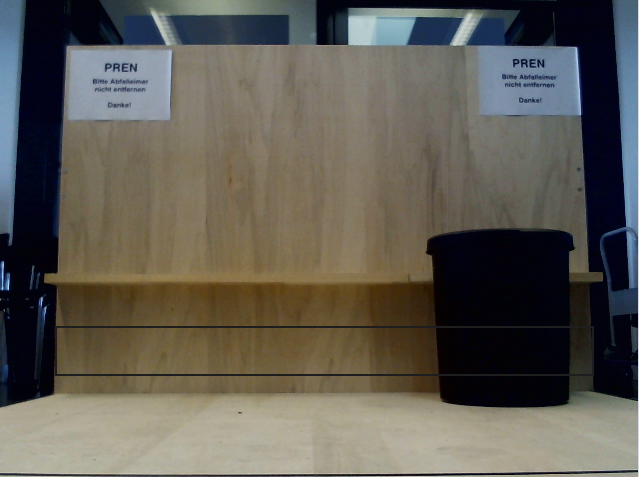
\includegraphics[width=1\textwidth]{fig/BildMitKorb_markiert.png}
	\caption{Bilderkennung - Ausschnitt}
	\label{fig:Bilderkennung_ausschnitt}        
\end{figure}

Der Ablauf der Bilderkennung funktioniert folgendermassen:
\begin{itemize}
	\item Der Bildausschnitt wird in ein schwarz/weiss Bild umgewandelt.
	\item Ein Algorithmus scannt den Bildausschnitt Zeile für Zeile.
	\subitem Es wird oben Links im Bildausschnitt gestartet.
	\subitem Es wird Pixel für Pixel durchgelaufen und das erste weisse Pixel gespeichert.
	\subitem Das Endpixel wird bestimmt, wenn auf das weisse Pixel ein schwazes Pixel folgt.
	\subitem Von den Start und Endpunkte über die verschiedenen Zeilen wird der Mittelwert berechnet.
\end{itemize}

\begin{figure}[h!]          
	\centering             
	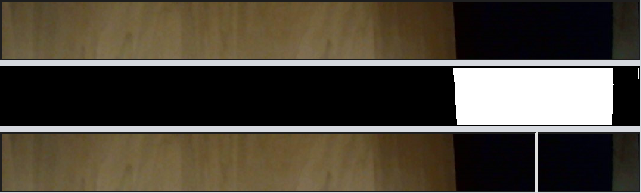
\includegraphics[width=1\textwidth]{fig/Korberkennung_Schritte.png}
	\caption{Bilderkennung - Ablauf}
	\label{fig:Bilderkennung_ablauf}        
\end{figure}

Mit dem gefundenen Mittelwert kann anhand von Geometrie der Winkel von der Maschine zum Korb bestimmt werden.
Es tritt ein Problem bei der Winkelbestimmung auf, falls der Korb sich links oder rechts am Rand befindet.
Da der Blick der Kamera kegelförmig ist, wird nicht der gesammte Korb erfasst. Die äussere Hälft des Korbs fehlt
und dies führt dazu, dass der Winkel zu klein ist. Das Problem wird behoben, indem bei der Überschreitung eines
Maximalwertes, der Winkel um ca. ein Grad erhöht wird.
